\documentclass[ecp,tc,english]{inputs/iiufrgs}

\usepackage[utf8]{inputenc}   % pacote para acentuação

\usepackage{graphicx}           % pacote para importar figuras
\usepackage{svg}

\usepackage{times}              % pacote para usar fonte Adobe Times
\usepackage{verbatim}

\usepackage{pdfpages} % usado no anexo, para incluir arquivos PDF inteiros.
\usepackage{adjustbox} % usado numa tabela que ficou muito larga

\usepackage{csquotes}
\usepackage{hyperref}
\usepackage[hyperref=true,style=abnt,repeatfields=true]{biblatex}
\usepackage{float} 
\addbibresource{biblio.bib}

\title{Procedural generation of cave-like maps for 2D top-down games}
\author{Milani Rodrigues de Freitas}{Vinicius}
\advisor[Prof.~Dr.]{Couto Barone}{Dante Augusto}
\coadvisor[Dr.]{Batista Silva de Carvalho}{Leonardo Filipe}
\date{}{2021}
\location{Porto Alegre}{RS}

\makeatletter

\let\newtitle\@title
\let\newauthor\@author
\let\newdate\@date
\makeatother

\sloppy

\begin{document}

\setcounter{page}{1}
\thispagestyle{empty}
\phantomsection
\pdfbookmark[1]{Cover}{cover}
\begin{center}
\setstretch{1.0}{
UNIVERSIDADE FEDERAL DO RIO GRANDE DO SUL\\
INSTITUTO DE INFORMÁTICA\\
CURSO DE ENGENHARIA DE COMPUTAÇÃO
}
\end{center}

\vfill

\begin{center}
VINICIUS MILANI RODRIGUES DE FREITAS
\end{center}

\vfill

\noindent\parbox[t]{\textwidth}{%
\centering%
\vbox to 20mm{%
\parbox[b]{90mm}{%
\centering\vbox to 50mm{%
        {\large\textbf{\@\newtitle}\par}
        \vfill
}}%
}}

\vfill

\vfill

\begin{center}
\setstretch{1.0}{
Porto Alegre\\
2021
}
\end{center}



\keyword{video game}
\keyword{procedural generation}
\keyword{dungeon}
\keyword{Unity}
\keyword{cave}

\maketitle

% agradecimentos
\clearpage
\begin{flushright}
\mbox{}\vfill
{\sffamily\itshape
Dedico este trabalho à minha família, amigos e namorada.
}\end{flushright}


\chapter*{Acknowledgements}

First, I would like to thank my advisor Dante Augusto Couto Barone for accepting my work proposal, for guiding me through the many changes we had, for connecting me to the right people and for his incredible availability and for being always helpful. I also would like to thank my co-advisor Leonardo Filipe Batista Silva de Carvalho for the great support and crucial help. 

I'd like to thank Anderson Ferrugem and Raphael Campos for participating in some of our meetings and providing essential information for this work.

Even though I ended up changing the work idea I started with them, I'd like to thank my former advisor Lisandro Zambenedetti Granville and my former coadvisor Lucas Bondan for their understanding.

I'd like to thank my parents Nei and Nelci for always being supportive of me, helping and encouraging me to achieve all my goals in life. I'm also thankful for the emotional support and encouragements of all of my friends, and last but not least, my girlfriend Débora Alexia, who was always there for me during the development of this work.
\clearpage

% EPÍGRAFE
\begin{flushright}
\mbox{}\vfill
{\sffamily\itshape
``quote.''\\}
--- \textsc{quem fez quote}
\end{flushright}

% palavras-chave
% iniciar todas com letras minúsculas, exceto no caso de abreviaturas

% Keywords precisam estar definidos ANTES do \maketitle

\begin{abstract}

Procedural Content Generation (PCG) has been extensively used in game design. With it, game content can be created automatically with limited or indirect user input. This application of PCG is important in lowering the cost and time-consumption of game design, specially in current years since the video-game industry has been experiencing a dramatic growth over the last decades. The objective of this work is to create a system that generates cave-like maps for 2D top-down games, which can serve as a blueprint for game designers to build upon on the future. Additionally, the work intends to evaluate if the generated maps have a set of qualities to make them be perceived as good or desirable by players. The system was developed in the Unity Game Engine, utilizing the C\# language and a combination of algorithms, that are presented and explained in this work. In order to evaluate the maps, criteria on what makes a good map were researched, and then applied a survey to test if the generated maps satisfied said criteria. A pretest questionnaire was made and answered by 23 participants, its results were used to develop an improved version of it, which was then answered by 163 participants. Finally, 9 out of 12 questions of the survey have reached their desired result.
\end{abstract}

\begin{englishabstract}
{Geração procedural de mapas de cavernas para jogos 2D top-down}
{Jogo eletrônico, geração procedural, calabouço, Unity, caverna}

A Geração Procedural de Conteúdo (PCG) tem sido amplamente utilizada no design de jogos eletrônicos. Com sua utilização, o conteúdo de um jogo pode ser criado automaticamente, através do uso de entradas de usuário limitadas ou indiretas. Esta aplicação de PCG faz-se importante para reduzir o custo e o consumo de tempo do design de jogos, especialmente nos anos atuais, já que a indústria de videogames sofreu um crescimento significativo nas últimas décadas. O objetivo deste trabalho é criar um sistema que gere mapas semelhantes a cavernas para jogos 2D top-down, que podem servir como uma base de desenvolvimento para designers de jogos. Além disso, o trabalho pretende avaliar se os mapas gerados possuem um conjunto de qualidades para que sejam percebidos como bons ou desejáveis pelos jogadores. O sistema foi desenvolvido utilizando-se do motor de jogos Unity, da linguagem C\# e de uma combinação de algoritmos, que são apresentados e explicados neste trabalho. Para avaliar os mapas, pesquisou-se por critérios sobre o que constitui um bom mapa e, em seguida, uma pesquisa foi realizada através de um questionário para testar se os mapas gerados satisfazem esses critérios. Um questionário de pré-teste foi aplicado e respondido por 23 participantes, seus resultados foram utilizados no desenvolvimento de uma versão aperfeiçoada deste, que foi respondida por 163 participantes. Por fim, 9 das 12 questões alcançaram seus resultados desejados.

\end{englishabstract}





% lista de figuras
\listoffigures

% lista de tabelas
\listoftables

% lista de abreviaturas e siglas
% o parametro deve ser a abreviatura mais longa

\begin{listofabbrv}{SPMD}
  \item[AI] Artificial Intelligence
  \item[CA] Cellular Automata
  \item[DFS] Depth-First Search
  \item[IMMS] Instructional Materials Motivational Survey
  \item[NPC] Non-Playable Character
  \item[PCG] Procedural Content Generation
  \item[RPG] Role-Playing Game
\end{listofabbrv}

% idem para a lista de símbolos
%\begin{listofsymbols}{$\alpha\beta\pi\omega$}
%       \item[$\sum{\frac{a}{b}}$] Somatório do produtório
%       \item[$\alpha\beta\pi\omega$] Fator de inconstância do resultado
%\end{listofsymbols}

% sumario
\tableofcontents



\chapter{Introduction} %fazer virar uma introduction
\label{chapter:intro}

Designing a game involves a conjunction of many different disciplines, for example: art, animation, sound, story, character creation, etc. Although the term game design is widely used in the industry to refer only to the design of the gameplay aspect, all the separate parts of design must properly work together in order to provide the player with a good experience \cite{zubek:2020}.

In this chapter we are going to present the necessary background information in order to understand what motivated this work. First, we will discuss the concept of game design and how it evolved through the ages. Then we will present some information about the game industry and the costs of developing a game. Lastly we will explain what procedural content generation (PCG) is and show a division of categories to better understand it.

After the motivation of the work is explained, we will present our objectives and preface the content of the next chapters. 

\section{Game design}

The importance of game design has increased throughout video game history. Designers of early games like Pong, shown here on Figure \ref{fig:pong}, or Spacewar! had very limited computing resources to work with, therefore it makes sense that they are simple and straightforward. Such games had little to no audio output, very primitive graphics and simple gameplay, sometimes borrowing ideas from well-established games, such as Pong, which is an electronic version of the Tabletennis sport \cite{wolf:2007}.

\begin{figure}[h]
    \caption{Atari's PONG arcade released in 1972}
    \centerline{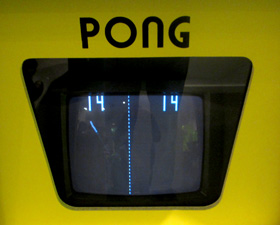
\includegraphics{images/introduction/PongScreenAtariOriginal.jpeg}}
    \legend{Source: \cite{pongmuseum:2021}}
    \label{fig:pong}
\end{figure}

In time, the technological advances made possible for more complex games to be created. Designing a game became much more nuanced and time consuming. 

\subsection{Evolution of the video game industry}

In 2020, the video game industry was already bigger than the movie industry and North American sports combined. The gaming industry has also experienced a big growth thanks to the COVID-19 pandemic \cite{marketwatch:2019}, since players are having more time at home for their hobby. But even before the pandemic, the industry was already in fast-grow along the last decades, as shown in Figure \ref{fig:growth_graph}.

\begin{figure}[h]
    \caption{Video game industry revenue through the ages}
    \centerline{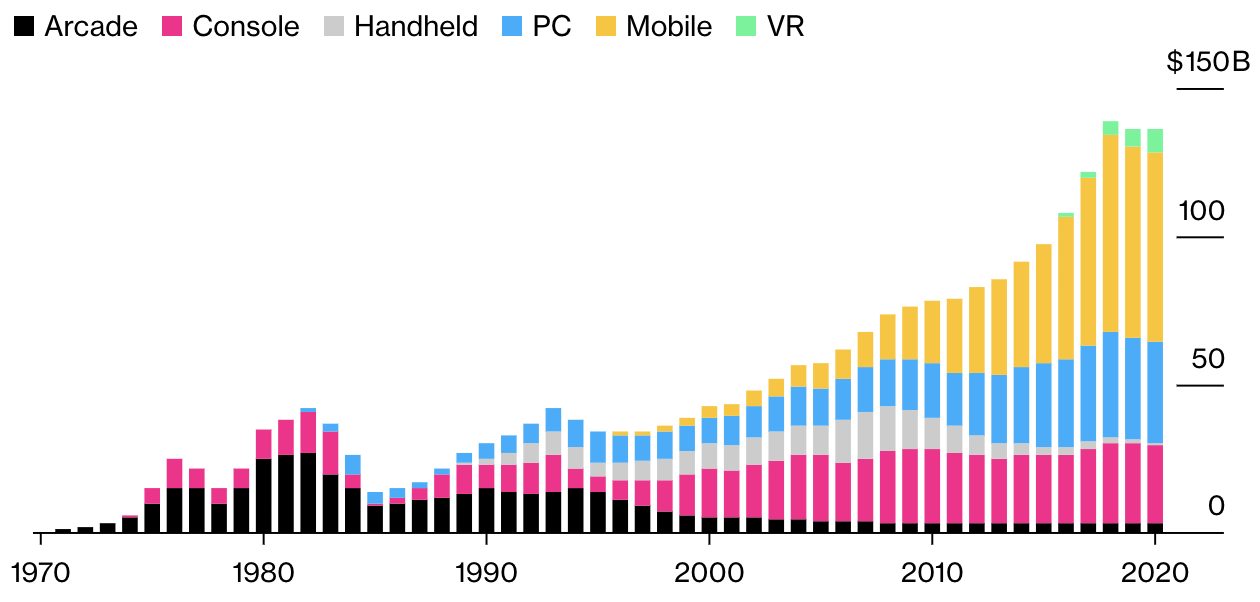
\includegraphics[width=13cm]{images/introduction/industry_growth.png}}
    \legend{Source: \cite{bloomberg:2019}}
    \label{fig:growth_graph}
\end{figure}

On the other hand, the cost of making games has increased dramatically as well. The cost of making Final Fantasy 7 remake, which was released in April 2020, for example, was roughly \$200 million, around \$120 million more than the original Final Fantasy 7, which was released in January 1997 \cite{cbr:2021}.

Triple-A games, which are games that are produced by mid-sized or major publishers \cite{steinberg:2007}, currently require the work of hundreds of people over the period of years to develop a single game. This is resulting in games not being as profitable for some developers, as few companies can afford developing long, diverse and polished games \cite{shaker:2016}.

One of the methods to reduce the cost of game designing is Procedural Content Generation (PCG), which uses algorithms to generate automatic content for the game.

\section{Procedural content generation}
\label{sec:pcg}

In the context of video games, PCG is defined as "the algorithmic creation of game content with
limited or indirect user input" \cite{togelius:2011}. In other words, PCG refers to software that is able to create game content by itself.

According to \textcite{doull:2008} there are 7 categories of PCG in games:

\begin{itemize}
\item \textbf{Runtime random level generation}: the generation of game levels while the game is being played. This is what people often think of when PCG in games is mentioned. In this category, an algorithm is responsible for generating random or pseudo-random levels for the game.

\item \textbf{Design of level content}: in this method, the automatically generated content is used at the level design stage to supplement human design skills. An algorithm can, for example, populate an environment created by the designer rapidly. Or the designer may choose specific generated levels to expand on.

\item \textbf{Dynamic world generation}: This technique is used to dynamically grow the environment that the player interacts on by using random seeds. In this case, the generated maps are never held in memory except as temporary structures to display.

\item \textbf{Instancing of in game entities}: in order to reach a statistically insignificant chance of repetition, in-game entities, such as like monsters, items, non-playable characters (NPCs), have some of their properties procedurally generated. These properties may be, for example, the position of the entity, its size, structure, etc.

\item \textbf{User mediated content}: this is a type of procedural generation where the user is in control. The technique offers a range of possibilities to users, who are responsible for putting them together in order to generate content.

\item \textbf{Dynamic systems}: some real-world systems such as group or weather behavior can be modelled using PCG techniques. This is widely used in combination of artificial intelligence (AI) in order to, for example, make NPCs react differently according to certain weather conditions.

\item \textbf{Procedural puzzles and plot generation}: this category is about using PCG in order to generate individual puzzle elements to increase replayability, e.g. changing door codes. Games that have its plot generated by PCG are also included in this category.
\end{itemize}

An example of a commercial game that was developed utilizing different PCG techniques is Electronic Arts's Spore. In this game, the player's objective is to evolve its own species, starting all the way from a microscopic organism until interstellar exploration. Entities on the game are generated by other players using in-game editors, which is an example of user mediated content generation. Worlds and galaxies are created through a combination of dynamic world generation and runtime random level generation. Moreover, some of the character animations are created procedurally \cite{wright:2007}. Figure \ref{fig:spore} shows user-generated characters standing on a procedurally generated world.

\begin{figure}[h]
    \caption{Screenshot of Spore gameplay}
    \centerline{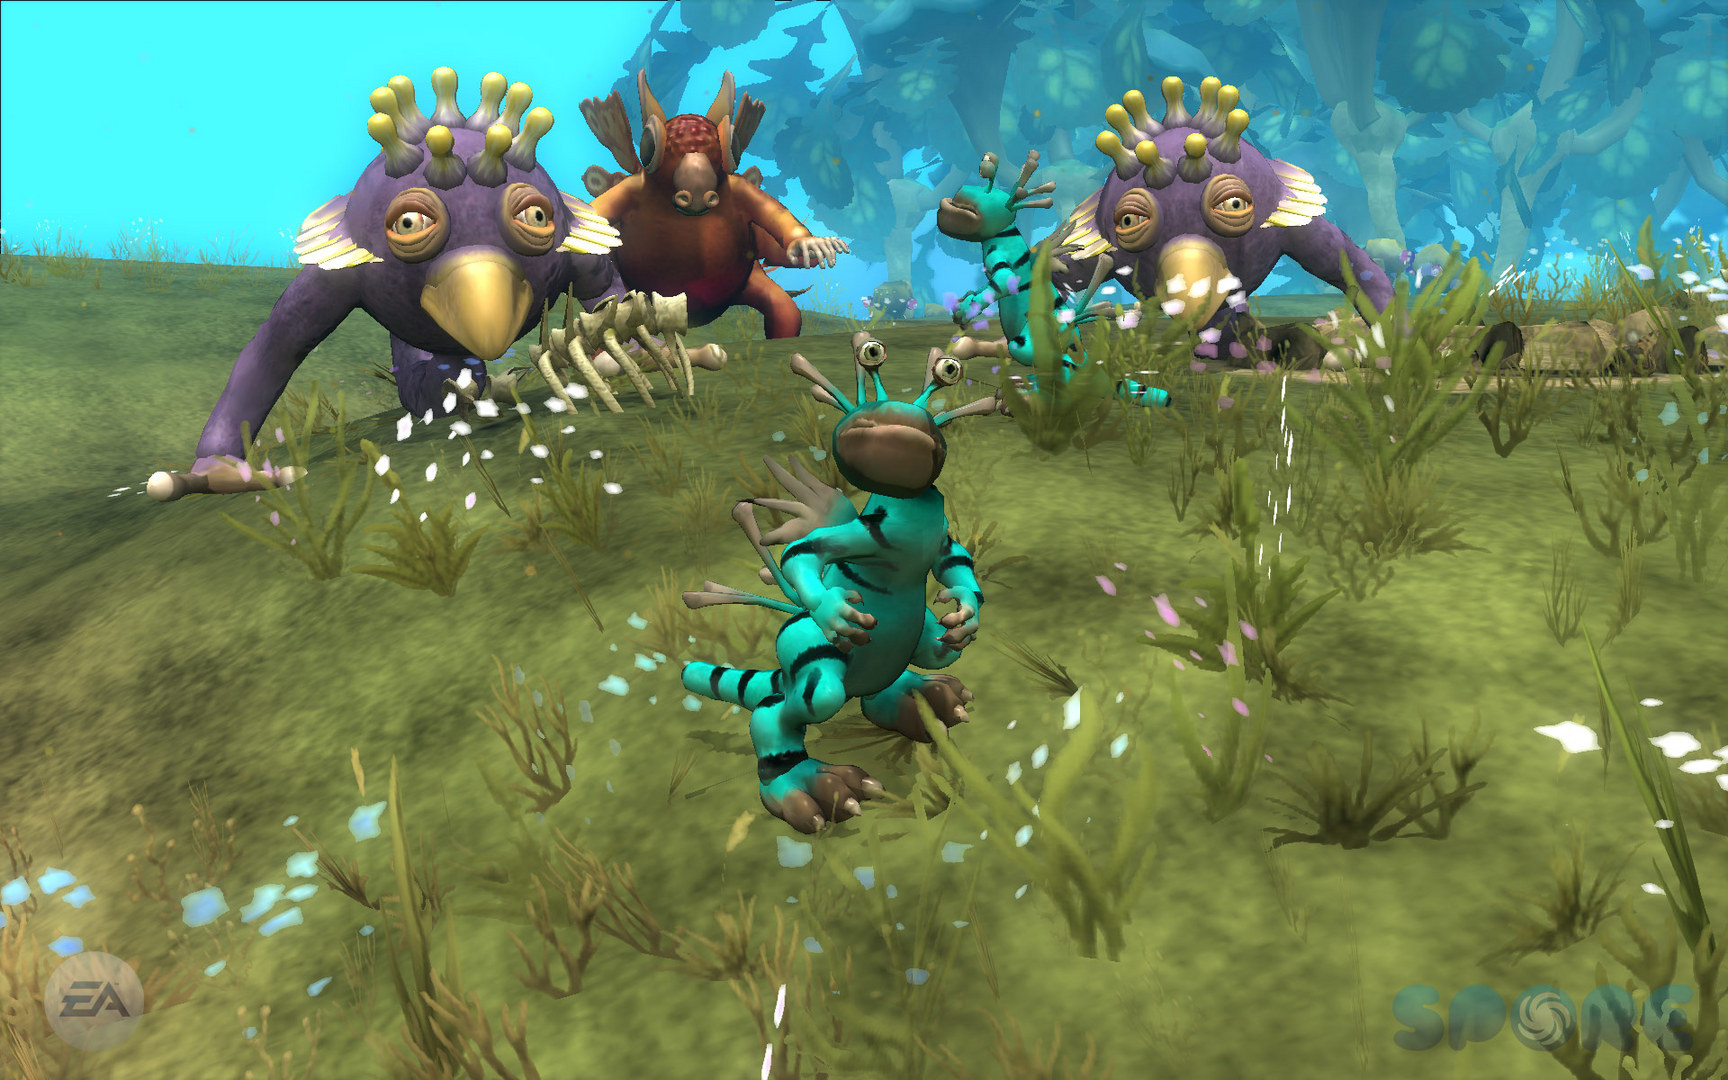
\includegraphics[width=13cm]{images/introduction/spore.jpg}}
    \legend{Source: \cite{ea:2008}}
    \label{fig:spore}
\end{figure}


\section{Dungeons in games}

One of the most notable applications of PCG in games is the creation of procedurally generated dungeons. A dungeon is a labyrinthic environment that the player can explore, as well as collect items, slay monsters, fall into traps, etc. Although originally the term "dungeon" refers to a labyrinth of prison cells, nowadays, there are dungeons representing caverns, castles, forests, underwater environments, etc \cite{shaker:2016}. 

This current definition of a dungeon can be probably tracked to the Dungeons and Dragons game, which is a tabletop Role-Playing Game (RPG) that had a huge influence in the development of video games throughout history. In fact, a specific type of computer RPG has spawned from the idea of exploring randomly generated dungeons: the roguelike genre. The name "roguelike" comes from the 1980's game Rogue, which featured procedurally generated dungeons that the player had to explore in search of an amulet \cite{brewer:2016}. A screenshot of a typical Rogue session can be seen in Figure \ref{fig:rogue}.

\begin{figure}[h]
    \caption{Screenshot of Rogue gameplay}
    \centerline{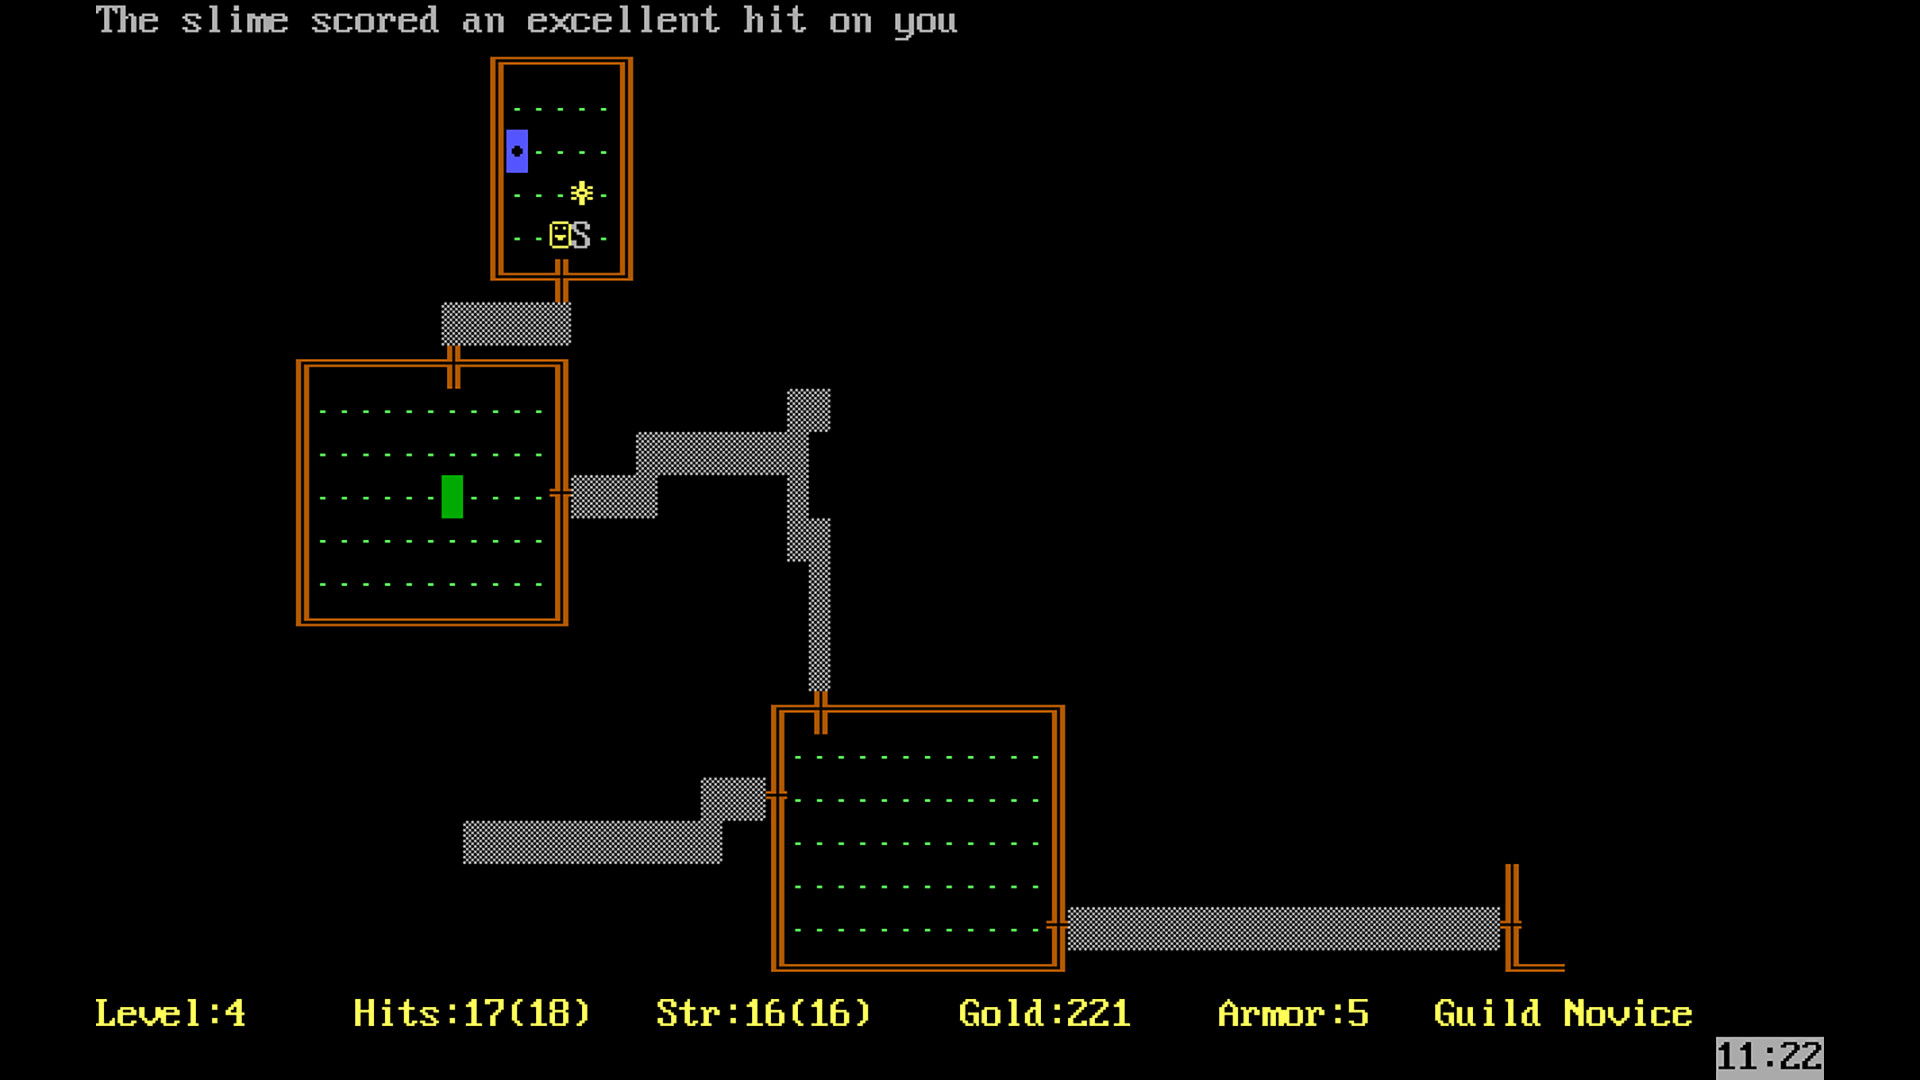
\includegraphics[width=13cm]{images/introduction/rogue.jpg}}
    \legend{Source: \cite{epyx:1985}}
    \label{fig:rogue}
\end{figure}

In \textcite{melan:2006} it is suggested that the design of the dungeon structure is very important to the creation of a good dungeon map. According to the author, a good map design is one that embodies the factors that make playing on a dungeon fun: exploration, decision making, consistent pace of action, discovery of secrets. Four different basic forms of dungeon maps, created from the author experience with RPG, were presented in \textcite{melan:2006},  shown here on Figure \ref{fig:basic_dungeons}. 

\begin{figure}[h]
    \caption{Basic dungeon structures}
    \centerline{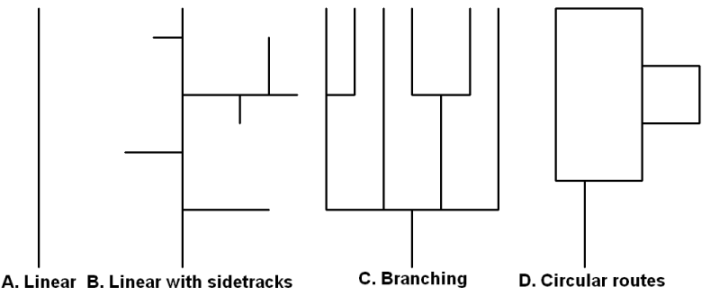
\includegraphics[width=13cm]{images/introduction/basic_dungeon.png}}
    \legend{Source: \cite{melan:2006}}
    \label{fig:basic_dungeons}
\end{figure}



\section{Objectives}
\label{sec:objectives}

Taking motivation from the information presented in the previous sections, this work has been elaborated with the objective of creating a PCG system to design cave-like dungeon maps for 2D top-down games.

More specifically, we will:

\begin{itemize}
\item \textbf{} Generate varied and cave-like dungeon maps from the combination of different algorithms.

\item \textbf{} Contribute to the PCG category of 'design of level content' by generating levels that can serve as a blueprint for game designers to build upon on the future.

\item \textbf{} Provide maps based on a set of criteria found in bibliography for what is considered a good dungeon map.

\item \textbf{} Evaluate if the generated maps match the criteria through a survey applied to video-game players.

\end{itemize}

\section{Organization of this work}

Next, on Chapter \ref{chapter:related}, we will cover works that are related to this one. After that, on Chapter \ref{chapter:proposal} our proposal will be expanded on and some background information will be provided in order to fully understand it. Following that, on chapter \ref{chapter:dev} we will provide details on our development and implementation. Chapter \ref{chapter:survey} will cover the creation of the survey and its results. Lastly on Chapter \ref{chapter:conclusion} we will discuss the conclusions of our work.


\chapter{Related Work}

In the search for works related to this one, we searched for works that focused on dungeon or content generation specifically for games and also for works that had their focus on cave generation.

\section{Conditional Convolutional Generative
Adversarial Networks Based Interactive
Procedural Game Map Generation}

This paper by \citeauthor{ping:2020} suggests the usage of Conditional Generative Adversarial Network and Convolutional Neural Network to create a game design system. The system takes by input a gameplay area map defined by the user and generates a complex map with the same design pattern.

\begin{figure}[h]
    \caption{Example of the system's usage}
    \centerline{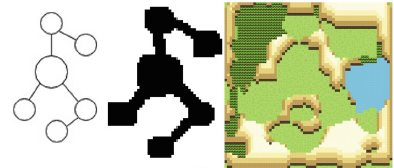
\includegraphics{images/related_work/ping.png}}
    \legend{Source: \cite{ping:2020}}
    \label{fig:ping}
\end{figure}
In Figure \ref{fig:ping} we see in the first two steps the image designed by the user and in the last step the generated map. The variety of the maps depend on the training of the network as well \citeyear{ping:2020}.

\section{Cellular automata for real-time generation
of infinite cave levels}

In this paper a simple cellular automata (CA) algorithm is used in order to generate, in real time, infinite cave-like levels. The algorithm was tested in a game called Cave Crawler, which is a birds-eye view game where the players have to traverse the generated tunnels while defeating waves of enemies. 

Much like this paper, our work also utilizes a simple CA algorithm as one of the steps of the system in order to generate the cave levels, but on this paper the focus is more on the real-time and performance aspect of the map generation \cite{johnson:2010}.

\section{Procedural creation of 3D solution cave models}

The focus of this article by \citeauthor{boggus:2009} is to use PCG algorithms to create 3D cave models based on real cave patterns. They present the usage of surface images of cave patterns and apply these images to create models of cave systems. The surface images can be generated, for example by utilizing fractal algorithms, or real world terrain data.

After the surface image is provided, they create a heightmap out of it and then simulate the flow of water through this map, since this is ultimately the way solution caves are formed. Figure \ref{fig:3d_cave} shows a cross section view of a generated cave, where lighter areas represent walls \citeyear{boggus:2009}.
\begin{figure}[h]
    \caption{Spongework cave pattern}
    \centerline{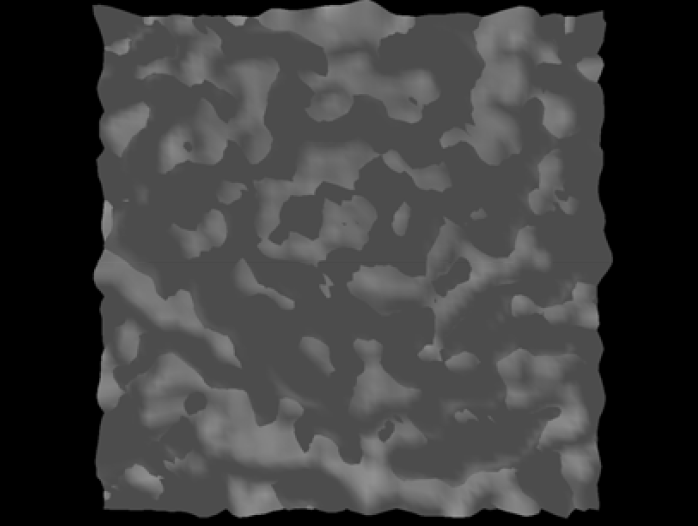
\includegraphics[width=7cm]{images/related_work/3d_cave.png}}
    \legend{Source: \cite{boggus:2009}}
    \label{fig:3d_cave}
\end{figure}

\section{Procedural Playable Cave Systems
based on Voronoi Diagram and Delaunay Triangulation}

This paper by \citeauthor{santamaria:2014} presents a new method for 2D or 3D playable cave systems to be generated. The user-defined input for their method are a list of points of interest (POI) that will be put inside the cave and the relationship between these POI. The paper defines a list of parameters that compose the POI like location, depth, number of branches etc.

\begin{figure}[h]
    \caption{Cave generation process}
    \centerline{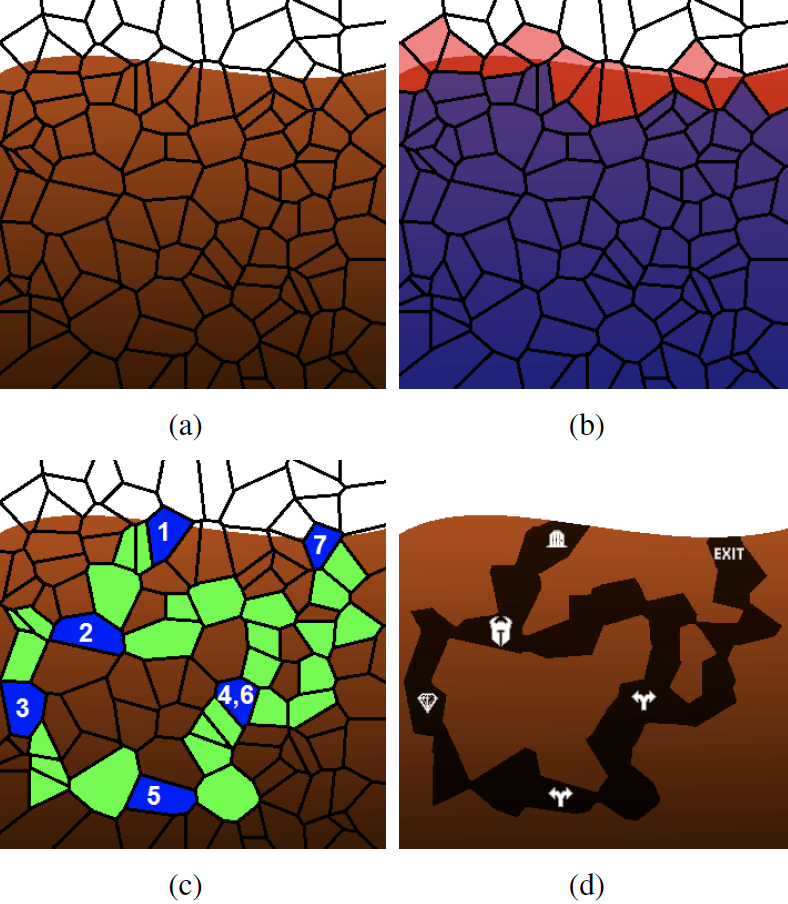
\includegraphics[width=6cm]{images/related_work/poi_cave.png}}
    \legend{Source: \cite{santamaria:2014}}
    \label{fig:poi_cave}
\end{figure}

Figure \ref{fig:poi_cave} shows their cave generation process. In (a) a Voronoi diagram is generated on a terrain representation. (b) shows the classification of the cells. (c) shows 7 POI assigned to their respective cells in the diagram and (d) shows the final generated cave \citeyear{santamaria:2014}.

\section{Analysis and Development of a
Game of the Roguelike Genre}

This work describe the development of a prototype game of the roguelike genre, and presents an analysis focused on the different techniques used on the AI for enemies and on the procedural generation of the dungeons. The compared PCG algorithms include: Kruskal and Prim, both being genetic algorithms; depth-first search, used to generate perfect mazes and cellular automata for cave-like structures. Some of the gathered results show that techniques of basic interaction iteration and BSP trees have good scalability while cellular automata and depth-first search need optimization or restriction in other to increase scalability \cite{goncalves:2015}.

\chapter{Proposal}
\label{chapter:proposal}

In this chapter we will define some concepts that will be necessary to fully understand our proposal that was developed in order to achieve the objectives presented in section \ref{sec:objectives}. In the last section we will expand on the criteria for what makes a good video-game map.

\section{Video-game maps}

In the context of video games, a map corresponds to a game scenery inhabited by the player and other entities like monsters, NPCs, objects etc \cite{carvalho:2011}. The specific type of map that we have selected in this work is the 2D top-down type. This map perspective, also sometimes referred to as overhead view, bird's-eye view, Godview etc, have a camera angle that shows the player and the area around them from above. An example of a game with an overhead view is shown in Figure \ref{fig:pokemon}.

\begin{figure}[h]
    \caption{Screenshot of Pokémon Gold gameplay}
    \centerline{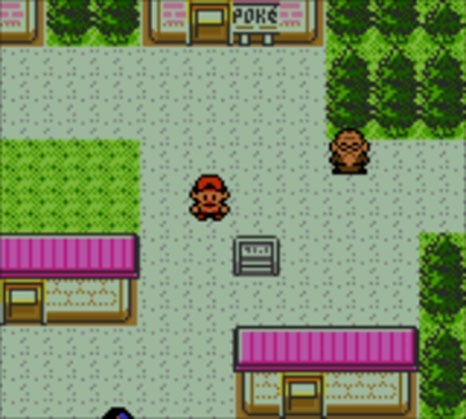
\includegraphics[width=6cm]{images/proposal/pokemon.png}}
    \legend{Source: \cite{pokemon:1999}}
    \label{fig:pokemon}
\end{figure}

\subsection{Map elements}

The tool chosen to develop our solution is the Unity game engine, which was released in 2005 and developed by Unity Technologies \cite{unity:2021}. Figure \ref{fig:unity_print} shows a screenshot of this tool with some important elements that will be described on the next items of this section. The description of such elements have been adapted from \cite{carvalho:2011}.

\begin{figure}[h]
    \caption{Screenshot of the Unity engine}
    \centerline{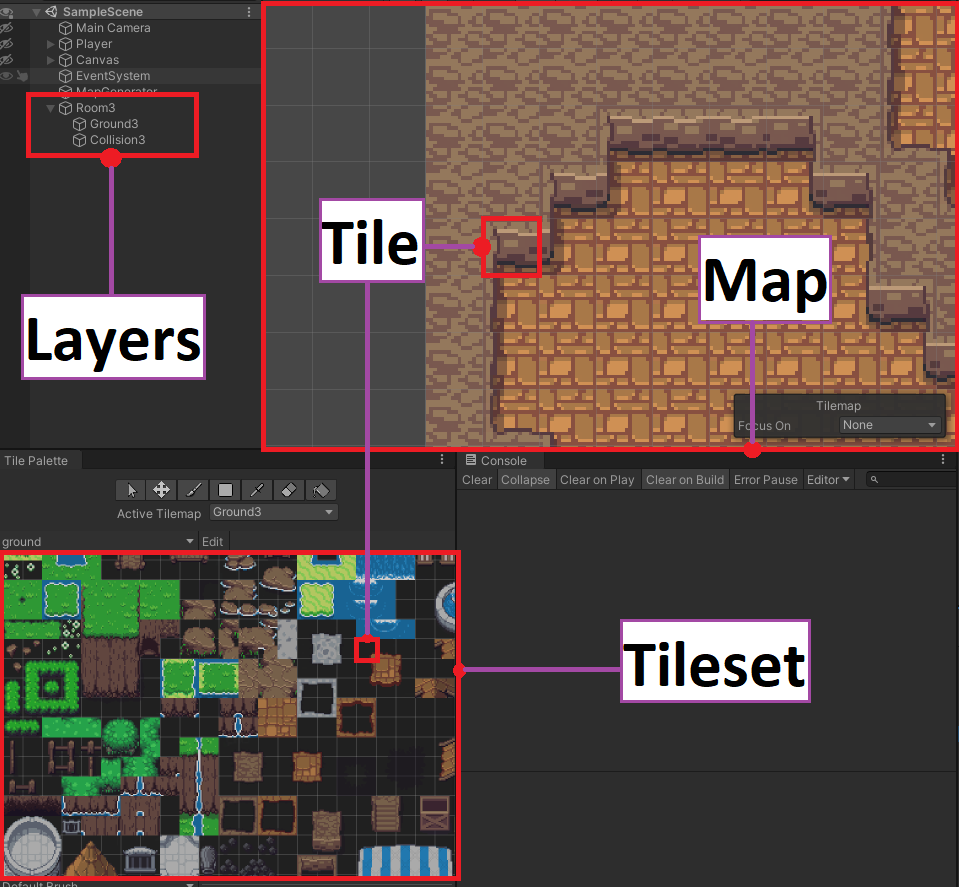
\includegraphics[width=11cm]{images/proposal/unity_print.png}}
    \legend{Source: Image provided by author}
    \label{fig:unity_print}
\end{figure}

\subsubsection{Map}
The map is represented here by a three-dimensional mesh of width \(w_{map}\) and height \(h_{map}\), with \{\(w_{map}, h_{map} \in \mathbb{N}|(w_{map}>0)\wedge(h_{map}>0)\)\}. Additionally, this mesh has a depth of \(l_{map}\) layers, with \{\(l_{map} \in \mathbb{N}|l_{map}\geq 1\)\}, in our specific case, \(l_{map} = 2\).

The map is composed by a number of \(w_{map} \times h_{map}\) cells, in our case each cell has one or two tiles (which will be explained in a subsequent section) one per layer, creating what is called a tiled map. 

\subsubsection{Layers}
The layers are the different levels of the map where it's elements are distributed. In the scope of this work, there are two types of elements that will compose our maps, they are: ground and walls. The ground is the path where the player can walk on, and the walls are what define the structure of the cave maps and the player cannot walk on them. Therefore these two elements are organized in two separate layers, here called ground layer and collision layer. The collision layer is named as such because, in order to avoid letting the player walk on the walls, a collider\footnote{In the Unity engine, the collider component is added to GameObjects where there's need to simulate physical collision.} component was added to this layer.

\subsubsection{Tiles}

A tile is the entity that occupy the cells of the map mesh. Each tile is an image that represents some object to be inserted in the game, this image is of dimensions \((i*w_{cel})\times(j*h_{cel})\) with \(w_{cel}\) and \(h_{cel}\) representing, respectively, the width and height of a cell in the map, and \(i\) and \(j\) are constants where \{\(i, j \in \mathbb{N}|(1\leq i<w_{map})\wedge(1\leq j<h_{map})\)\}. In our specific case, \(w_{cel}=h_{cel}=16 {pixels}\) and all tiles used have \(i=j=1\). 
\subsubsection{Tileset}

A tileset is, as the name suggests, an image containing the set of tiles that will represent the game objects.

The Unity engine divides the given tileset into a number of tiles that can be used by the developer to fill the map mesh and create an envinronment. The tileset used on this work is the "Zelda-like tileset", which was posted by \citeauthor{arm:2017} and is licensed in the public domain \citeyear{arm:2017}. Figure \ref{fig:tileset} shows the tileset, although only the tiles needed for walls and ground were used in this work, they will be shown in the next chapter.

\begin{figure}[h]
    \caption{Zelda-like tileset}
    \centerline{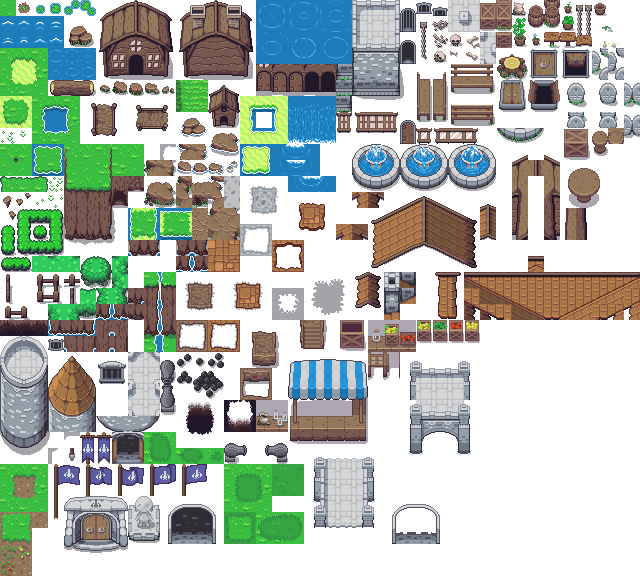
\includegraphics[width=10cm]{images/proposal/overworld.png}}
    \legend{Source: \cite{arm:2017}}
    \label{fig:tileset}
\end{figure}

\section{Cave patterns}

As will be discussed in the next section, one of the characteristics that make a good map is for it to have a natural look. Since we focused on cave-like maps, we researched for what would be a natural cave representation in a 2D top-down view.

According to \cite{audra:2011}, Figure \ref{fig:cave_patterns} show some of the most common cave patterns. They are formed by having different types of sources of water interacting with different kinds of soil.

\begin{figure}[h]
    \caption{Common cave patterns}
    \centerline{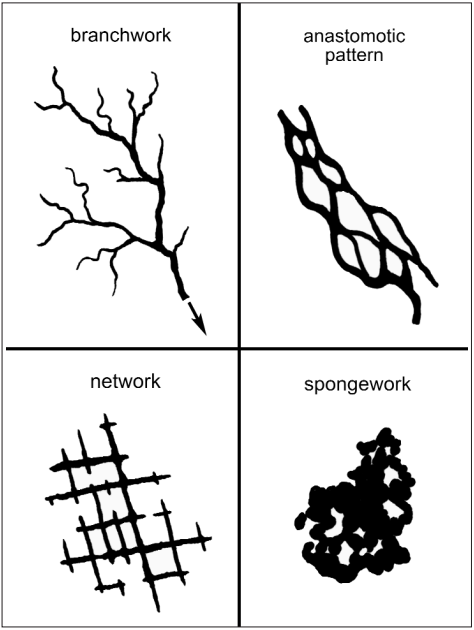
\includegraphics[width=6cm]{images/proposal/cave_patterns.png}}
    \legend{Source: \cite{audra:2011}}
    \label{fig:cave_patterns}
\end{figure}

It is outside of the scope of this work to give a larger description to each of the different cave patterns shown here, but it's important to note that this is an accurate representation of real-world caves and they were used as a reference for the generated maps.

\section{What makes a good generated map}
\label{sec:goodmap}

At last, an important part of our proposal is to generate maps that have a set of qualities that make them be perceived as good or desirable maps.

During the bibliographic research for these criteria, most of the findings related not only to the map but to the video-game level entirely, for example in \cite{preuss:2014} where the placement of enemies and treasures are also taken into consideration.

However, there were some criteria found that made reference only to the map itself. Here are the qualities of a good generated map, according to bibliographic research:

\begin{itemize}
\item The generated maps should have a natural look, they shouldn't look as if they were generated by an algorithm \cite{shaker:2016} \cite{adams:2002}.
\item Dungeon maps should have an entrance, an exit (sometimes being the same), and a path between them \cite{shaker:2016}.
\item The Generated maps should look different from one another, to provide the player with an unique experience each time \cite{goncalves:2015} \cite{zapata:2014}.
\item The generated maps should encourage players to explore \cite{ping:2020}.
\item Borders are necessary on the generated maps, in order to prevent players and monsters from escaping them \cite{torrado:2020}.
\end{itemize}

To evaluate if the generated maps have the qualities cited here, we created a survey based on the one used here \cite{carvalho:2016}, which was developed using the ARCS model by Keller. Therefore, some of the elements for a good map that we will be evaluating are also adapted from the components of the ARCS model:

\begin{itemize}
    \item \textbf{Attention}:
    \begin{itemize}
        \item The design of the generated maps should be able to keep the player attention on the game.
        \item The generated maps' design should be attractive to the players.
    \end{itemize}
    \item \textbf{Relevance}:
    \begin{itemize}
        \item The player should want to play a game that includes the generated maps.
    \end{itemize}
    \item \textbf{Confidence}: 
    \begin{itemize}
        \item The generated maps should not appear to be too hard for the player.
        \item When looking at the map, the player should be able to comprehend it easily.
    \end{itemize}
    \item \textbf{Satisfaction}:
    \begin{itemize}
        \item The player should want to explore the map.
    \end{itemize}
\end{itemize}

More information about the survey will be given in Chapter \ref{chapter:survey}.
%  por fim falar da proposta: gerar um bom mapa em unity, o que é um bom mapa,
\chapter{Implementation}


as partes da implementação blablabal

\chapter{Methodology of validation}
\label{chapter:survey}

This chapter will discuss the creation of the questionnaire that was applied to video-game players, the conduction of its pretest, leading to its revision and the application of its final version. After that, we will discuss the results obtained.

As mentioned on Section \ref{sec:goodmap}, a survey was developed in order to test if a number of our generated maps can achieve the criteria we defined for what is considered a good generated map, which was built by adapting the measured tool of the ARCS model available at \textcite{carvalho:2016}, originally used to assess the motivation of players to play a game. Both the questionnaire and its pretesting version were made available through Google Forms in Brazilian Portuguese. They make use of the typical five-level Likert scale \cite{likert:1932}:
\begin{itemize}
    \item Strongly disagree.
    \item Disagree.
    \item Neither agree nor disagree.
    \item Agree
    \item Strongly agree.
\end{itemize}

Both questionnaires start with a question about the participant age group, and a question about how familiar they are with 2D top-down games. Also in both cases, participants were asked to carefully visualize eight different maps generated by our system. These images are available in Appendix \ref{appendix:a}. The main concern during the generation of these maps was to create a variety of results by tuning the user-defined parameters of the system.

English versions of the questionnaires are available in Appendix \ref{appendix:b} and Appendix \ref{appendix:c}. The justification of each question is also presented. Details about both of them will be discussed in the next sections, as well as their results.
 
\section{Pretest questionnaire}

Before sharing a definitive version of the questionnaire, a pretest was made with a smaller group of participants, in order to determine the strengths and weaknesses of our survey concerning question format and wording.

The pretest had 23 participants. These were the first two questions, made with the purpose of understanding the profile of the respondents:
\begin{itemize}
    \item What is your age group (in years)?
    \begin{itemize}
        \item \emph{(18-)} Less than 18.
        \item \emph{(18 - 25)} Between 18 and 25.
        \item \emph{(26 - 30)} Between 26 and 30.
        \item \emph{(31 - 35)} Between 31 and 35.
        \item \emph{(35+)} More than 35.
    \end{itemize}
    \item How familiar are you with 2D top-down games? (games like Zelda, Pokémon, Bindings of Isaac, Hotline Miami etc)
    \begin{itemize}
        \item \emph{(1)} Never heard of it.
        \item \emph{(2)} Heard of it, but never played.
        \item \emph{(3)} I've seen videos of people playing this type of games.
        \item \emph{(4)} I've played at least one game in this style.
        \item \emph{(5)} I've played more than one game in this style.
    \end{itemize}
\end{itemize}

The results of these questions are shown here in Figure \ref{fig:pre_age} and Figure \ref{fig:pre_game}. We had the participation of mostly young people who were already familiar with the concept.

\begin{figure}[h]
  \centering
  \begin{minipage}[b]{0.4\textwidth}
    \caption{Age group of participants.}
    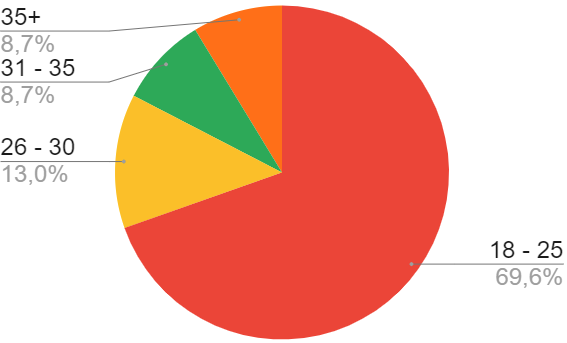
\includegraphics[width=\textwidth]{images/survey/pretest_age.png}
    \legend{Source: Image provided by author}
    \label{fig:pre_age}
  \end{minipage}
  \hfill
  \begin{minipage}[b]{0.4\textwidth}
    \caption{Participants' familiarity with 2D top-down games.}
    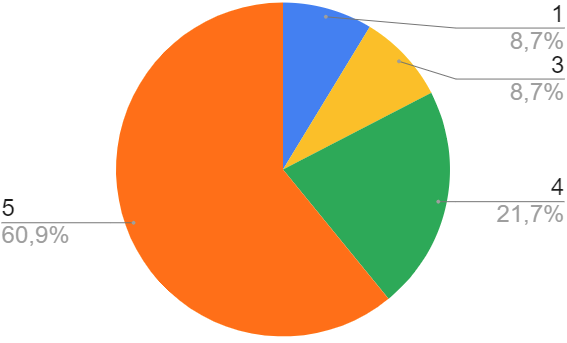
\includegraphics[width=\textwidth]{images/survey/pretest_played.png}
    \legend{Source: Image provided by author}
    \label{fig:pre_game}
  \end{minipage}
\end{figure}

After these initial questions, as mentioned before, participants were asked to carefully visualize the map images shown in Appendix \ref{appendix:a}, then they responded the 15 questions regarding the map, available in Appendix \ref{appendix:b}. Also, Appendix \ref{appendix:b} contains the next part of the pretest, which involves answering five subjective questions about the questionnaire itself, shown in Table \ref{table:pretest_quest}.

\subsection{Pretest results}

For the pretest, the results we analyzed are the ones about the questionnaire itself, i.e., the ones in Table \ref{table:pretest_quest}. All of the points listed here have been taken into account when developing the second version.

\subsubsection{Question 1}

Question 1 reads: "Do you think that the questions from this questionnaire were easy to understand? If not, why?".

This question had 12 answers, from which 7 were positive, 3 were negative and 2 were neutral. The most important points we gathered from the neutral and negative answers were:

\begin{itemize}
    \item Participants weren't sure what the map would be used for, this made it harder for them to answer the questions.
    \item Participants who were unfamiliar with 2D top-down games found it hard to visualize how the maps could be explored.
\end{itemize}

\subsubsection{Question 2}

Question 2 reads: "Are there repeated questions in this questionnaire? If yes, which?".

This question had 17 answers, from which 9 were negative and 8 were positive. All of the positive answers referred to questions that were opposites from one another, for example, question 9 (The generated map’s design made it difficult for me to keep my attention.) and 10 (The generated cave maps were capable of capturing my attention.).

\subsubsection{Question 3}

Question 3 reads: "Would you include other questions on this questionnaire? If yes, which?".

This question had 16 answers, from which 7 were negative and 9 were positive. Most of these 9 positive answers suggested some type of comparison between the maps. From our understanding, adding questions that compare the generated maps is beyond the scope of this work, therefore we concluded that we need to better explain the objectives of the work before asking the questions.

One of the suggestions was to add a demonstration of how a character would view these maps, how far away would the camera be, how much of the map could be seen etc. 

\subsubsection{Question 4}

Question 4 reads: "Would you change the text of one or more questions in this questionnaire? If yes, which?".

This question had 14 answers, from which 7 were negative and 7 were positive. The most important points gathered from the positive answers are listed below:
\begin{itemize}
    \item Grammatical errors to be corrected.
    \item Use of a more direct language.
    \item Change questions 7 and 8 so that, instead of measuring the influence of colors and textures compared to the structure of paths, we can measure the influence of each separately.
\end{itemize}

\subsubsection{Question 5}

Question 5 reads: "Do you think a question comparing the generated maps to real cave representation is necessary for this questionnaire?".

This question had 19 answers, from which 13 were positive and 6 were negative. Some of the positive answers suggested showing some real cave patterns, arguing that it can be difficult to imagine how the structure of a cave can be represented in 2D.

\section{Second version of questionnaire}

After reviewing all the suggestions and important points brought up on the pretest questionnaire, we developed an improved version of it, which can be seen on Table \ref{table:final_quest} of Appendix \ref{appendix:c}.

The second version had 163 participants, the first two questions were the same as the ones asked in the pretest and their results can be seen in Figure \ref{fig:age} and in Figure \ref{fig:gamekn}. We can see by these results that the participants' profile is the same as the one the pretest.

\begin{figure}[h]
  \centering
  \begin{minipage}[b]{0.4\textwidth}
    \caption{Age group of participants.}
    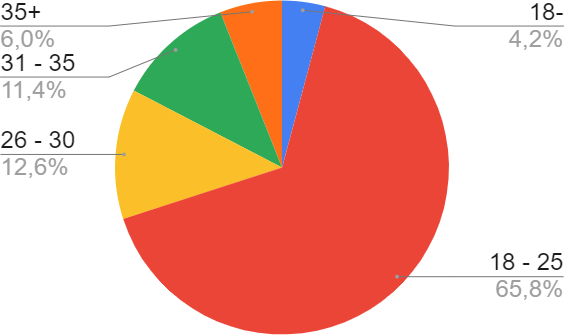
\includegraphics[width=\textwidth]{images/survey/age.png}
    \legend{Source: Image provided by author}
    \label{fig:age}
  \end{minipage}
  \hfill
  \begin{minipage}[b]{0.4\textwidth}
    \caption{Participants' familiarity with 2D top-down games.}
    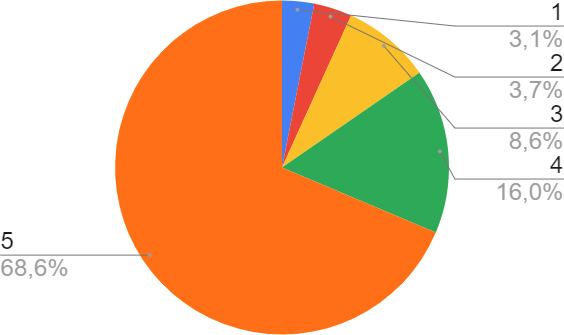
\includegraphics[width=\textwidth]{images/survey/played.png}
    \legend{Source: Image provided by author}
    \label{fig:gamekn}
  \end{minipage}
\end{figure}

A new question was added with the intent of better identifying the profile of the participants: "Did you ever participate in the development of a video game?". For which 41,1\% answered positively and 58,9\% answered negatively. This is relevant since, as discussed on Section \ref{sec:pcg}, one of the main objectives of PCG in video games is to assist in game design.

After these three initial questions, the participants were given a summary of the objectives of this work, along with the image from Figure \ref{fig:cave_patterns}, to assist in answering the questions to come. Additionally, an animated GIF of a character walking around one of the generated maps was added. A still image of this GIF can be seen here on Figure \ref{fig:gif}.

\begin{figure}[h]
    \caption{Still frame of GIF shown to participants, showing a character walking on a generated map.}
    \centerline{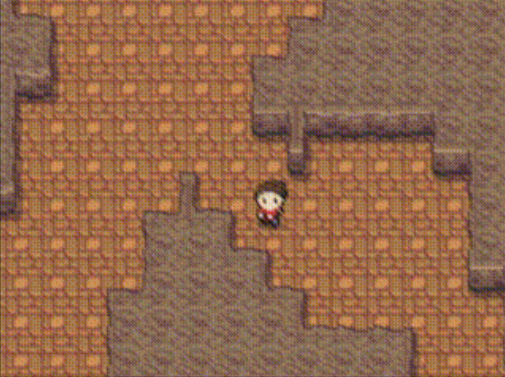
\includegraphics[width=8cm]{images/survey/gif.png}}
    \legend{Source: Image provided by author}
    \label{fig:gif}
\end{figure}

\subsection{Analysis of results}

The total results can be seen on Figure \ref{fig:final_res1}, where the questions that have the ideal response as \emph{Strongly agree} are marked with a \emph{(+)} after the question number, and the ones that have the ideal response as \emph{Strongly disagree} are marked with a \emph{(-)}.

\begin{figure}[h]
    \caption{Total results of the second version questionnaire.}
    \centerline{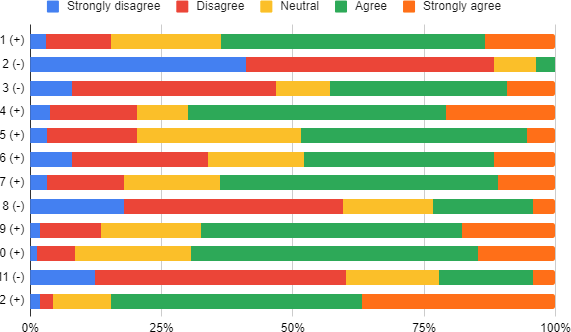
\includegraphics{images/survey/final_results_1.png}}
    \legend{Source: Image provided by author}
    \label{fig:final_res1}
\end{figure}

To analyze the results, we assigned a weight to each option of the Likert scale, from 1 (strongly disagree) to 5 (strongly agree). The question's proposition was considered satisfied if the average of answers achieved 60\% of the ideal value. For some questions the ideal is to reach 5, for others the ideal is to reach 1. Therefore, considering \(MAX\) as the maximum answer, \(MIN\) as the minimum answer, and \(V_{max}\) and \(V_{min}\) as the maximum and minimum satisfactory value, respectively:

\begin{center}
\(V_{max} = (MAX - MIN) * 0.6 + MIN = (5 - 1) * 0.6 + 1= 3.4\)
\(V_{min} = (MAX - MIN) * 0.4 + MIN = (5 - 1) * 0.4 + 1 = 2.6\)
\end{center}

The average and mode of the answers is shown on Figure \ref{fig:final_res}.

\begin{figure}[h]
    \caption{Average and mode of the second version questionnaire.}
    \centerline{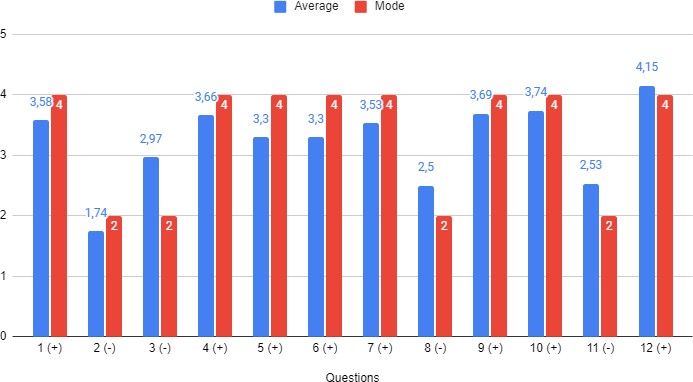
\includegraphics{images/survey/final_results.png}}
    \legend{Source: Image provided by author}
    \label{fig:final_res}
\end{figure}

By these metrics; questions 1, 2, 4, 7, 8, 9, 10, 11 and 12 have reached a satisfactory result; while questions 3, 5 and 6 have not.

Out of the questions that have reached satisfactory results, the most important points gathered were:
\begin{itemize}
    \item All of the questions related to the ARCS model for measuring motivation have reached satisfactory results.
    \begin{itemize}
        \item Attention was shown to be the least influential component (questions 1 and 8).
        \item Confidence and relevance were the major drivers for motivation (questions 2 and 12).
    \end{itemize}
    \item The structure of the caves was shown to be slightly more important in achieving the natural look for the map (question 7).
    \item The variety criteria didn't reach a very expressive result, although still below the 40\% mark (question 11).
    \item The criteria that proposed that the generated maps should encourage players to explore was reached by a good margin (question 9).
\end{itemize}

Out of the questions that haven't reached satisfactory results, the most important points gathered were:
\begin{itemize}
    \item It would be easy to get lost on the generated maps (question 3).
    \begin{itemize}
        \item This could be attributed to the labyrinthic nature of caves.
        \item Generating larger maps tend to create many branching paths. This can mean that the system is more effective when generating smaller maps.
    \end{itemize}
    \item Even though the results of question 4 suggests that the system can generate natural-looking structures, the result of question 5 suggests that the maps still don't quite look like real caves. Although the result was not drastically low. 
\end{itemize}
\chapter{Conclusion}
\label{chapter:conclusion}

This work showed how PCG is important in game design and how the price of game development has been increasing throughout the years, it proposed the development of a PCG system to generate good cave-like maps and finally it evaluated this system through a survey.

One of the biggest challenges faced was the research for criteria on what makes a good map, that can be seen on Section \ref{sec:goodmap} of Chapter \ref{chapter:proposal}. Most of the work we found focused on video-game \emph{levels}, which contain more elements like enemies and treasures. Due to this difficulty we decided to also include metrics from the ARCS model, taking inspiration from \cite{carvalho:2016}, and adapted them, since they are normally used to measure motivation in learning. In this sense, the evaluation method for generated maps proposed on this work can be reused by others.

The creation of the system required knowledge from different areas and the use and adaptation of many algorithms. The system had many user-defined parameters which is a positive in map generation, since a larger variety of maps can be created. Even though the work focused on cave-like maps, by changing the used tiles the system can generate maps like forests, open fields, rivers etc. Figure \ref{fig:river} shows a procedurally generated river, created with the use of the system.

\begin{figure}[h]
    \caption{River generated by the system.}
    \centerline{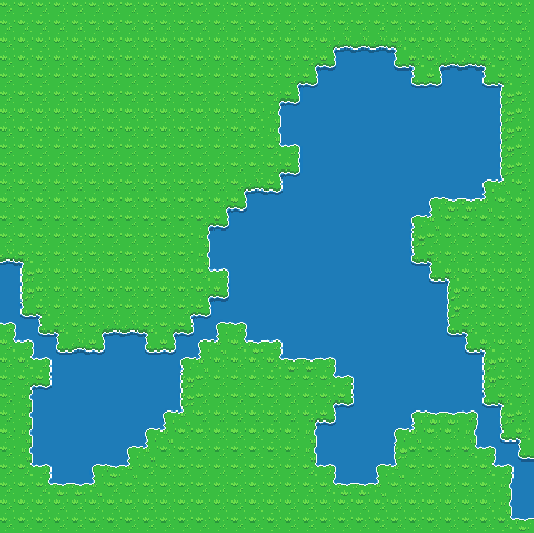
\includegraphics[width=6cm]{images/river.png}}
    \legend{Source: Image provided by author}
    \label{fig:river}
\end{figure}

The survey was answered by 163 participants, most of them from the age group that composes the average gamer, and most of them with familiarity to 2D top-down games. From the 12 questions, 9 achieved satisfactory results and 3 did not. Out of these results we found that the generated maps were successful in giving motivation. We also found that, even thought the structure of the maps resemble natural caves, the maps were not found to be much similar to 2D representations of real caves.

Finally, as a future works, the system could be turned into an Unity tool, that can then be used to create full games. The generation of rivers can be expanded on, by comparing them to real-life rivers and evaluating with a similar survey. The generation of maps can be changed to a level-generator, where the system wouldn't only generate the map but also place enemies, treasures, hidden passages etc.

\printbibliography

\end{document}
